% chercher des documents LaTeX dans styles, corps et bib
\makeatletter\def\input@path{{styles/}{corps/}}\makeatother

% Utiliser le style rapport.cls
\documentclass{rapport}


\title{Environnement de simulation pour ROVs}
\author{Quentin \textsc{Brateau} \\ \texttt{quentin.brateau@ensta-bretagne.org}}
\date{\today}
\doctype{Rapport de PFE}
\promo{Version 0.1}
\etablissement{\textsc{Ensta} Bretagne\\2, rue François Verny\\
  29806 \textsc{Brest} cedex\\\textsc{France}\\Tel +33 (0)2 98 34 88 00\\ \url{www.ensta-bretagne.fr}}
\logoEcole{
\includegraphics[height=4.2cm]{logo_ENSTA_Bretagne_Vertical_CMJN}}

\hypersetup{
  pdftitle={Rapport de PFE},
  pdfauthor={Quentin Brateau},
  pdfkeywords={guide, rapport de projet},
  bookmarksnumbered,
  pdfstartview={FitH},
  citecolor=blue,
  breaklinks=true
}

% creer le glossaire
\makeglossaries
% creer l'index
\makeindex

\begin{document}
	% Début du préambule
	\frontmatter
	% inclure la liste des acronymes
	\newglossaryentry{ENSTAB}{type=glo,
	text={\textsc{ENSTA} Bretagne},
	name={\textsc{ENSTA} Bretagne},
	description={Ecole Nationale Supérieure de Techniques Avancées Bretagne}}

\newglossaryentry{ROV}{type=glo,
	text={\textsc{ROV}},
	name={\textsc{ROV}},
	description={Remotely Operated Vehicles, véhicule sous-marin téléguidé}}

\newglossaryentry{Argos}{type=glo,
	text={\textsc{Argos}},
	name={\textsc{Argos}},
	description={\gls{ROV} commercialisé par Forssea Robotics}}

\newglossaryentry{Atoll}{type=glo,
	text={\textsc{Atoll}},
	name={\textsc{Atoll}},
	description={\gls{ROV} commercialisé par Forssea Robotics}}

\newglossaryentry{Navcam}{type=glo,
	text={\textsc{Navcam}},
	name={\textsc{Navcam}},
	description={camera de navigation réalisant un traitement temps-réel basé sur des algorithmes d'intelligence artificielle}}

\newglossaryentry{Obscam}{type=glo,
	text={\textsc{Obscam}},
	name={\textsc{Obscam}},
	description={camera d'observation}}

\newglossaryentry{frameLBL}{type=glo,
	text={\textsc{Frame lbl}},
	name={\textsc{Frame lbl}},
	description={Cadre portant des balise Long Baseline permettant la localisation sous-marine}}

\newglossaryentry{Gazebo}{type=glo,
	text={\textsc{Gazebo}},
	name={\textsc{Gazebo}},
	description={Logiciel de simulation multi-physique dédié à la robotique : \url{http://gazebosim.org/}}}

\newglossaryentry{ROS}{type=glo,
	text={\textsc{ROS}},
	name={\textsc{ROS}},
	description={Middleware dédié à la robotique : \url{https://www.ros.org/}}}

\newglossaryentry{Plugin}{type=glo,
	text={\textsc{Plugin}},
	name={\textsc{Plugin}},
	description={Module d'extension permettant d'ajouter des fonctionnalités à un logiciel}}

\newglossaryentry{Cpp}{type=glo,
	text={\textsc{C++}},
	name={\textsc{C++}},
	description={Language de programmation}}

\newglossaryentry{GSL}{type=glo,
	text={\textsc{GSL}},
	name={\textsc{GSL}},
	description={GNU Scientific Library, une librairie \gls{Cpp} permettant de résoudre des problèmes mathématiques}}
	% creer le titre ici
	\maketitle

	% chargement du fichier abstract.tex
	% 
\section*{R�sum�}
  Dans le cadre de ses fonctions, l'ing�nieur se doit de ma�triser les
  techniques de base de r�daction de documents.

  Le pr�sent guide fournit les premiers �l�ments visant � la r�daction d'un
  rapport de projet. Il est destin� aux �l�ves effectuant un projet dans le
  cadre de leur scolarit� � l'\gls{enstab}.  Sont pr�sent�s, de fa�on
  synth�tique, les bases sur la nature et la structure du rapport, ses r�gles
  de composition et de typographie.

\section*{Mots cl�s}
Rapport de projet, m�moire, r�daction.

\selectlanguage{english}
\section*{Abstract}
  In the context of their profession, engineers have to master basic
  techniques for writing documents.
  
  This guide provides the fundamental elements for writing a project
  report. It is intended for students undertaking projects during their
  studies at \gls{enstab} and it gives an overview of the basics in
  relation to the nature and components of a report, with formatting
  guidelines and typographic rules.
  
\section*{Keywords}
Project report, memoir, writing.

\selectlanguage{french}

\section*{Remerciements}

Je remercie Nathalie Debese, Amandine Nicolle, Olivier Reynet et H�l�ne Thomas
pour leur travail de relecture.


%%% Local Variables: 
%%% mode: latex
%%% TeX-master: "../guide"
%%% End: 


	\clearpage

	% table des matieres
	\tableofcontents

	\clearpage

	% Partie principale
	\mainmatter

	\chapter{Simulation de l'environnement}
\label{chapitre:environnement}
	
	\section{Introduction}

		La simulation de l'environnement est une partie importante du simulateur car c'est ce qui va définir le comportement des \gls{ROV}s dans leur milieu. Elle doit être très proche des conditions réelles afin d'avoir des résultats exploitables. Il faut donc établir les différents élements de l'environnements qui vont interagir avec les \gls{ROV}s afin de les intégrer dans le simulateur. Il y a principalement le milieu marin qui va ajouter une flottabilité au robots, mais aussi la présence de courants et enfin l'ombilical qui relie les \gls{ROV}s au bateau afin de l'alimenter en énergie mais aussi d'avoir un retour d'informations.

		La simulation de milieux marins est quelque chose de connu dans le domaine de la robotique. Il existe de nombreux simulateurs d'environnements marins et sous-marins~\cite{Manhaes_2016, bingham19toward, MARS, Rock}. Ces simulateurs proposent tous un modèle de flottabilité pour les objets à simuler, ce qui permet de pouvoir définir des bateaux ou bien des robots sous-marins. Cela permet donc de pouvoir simuler le comportement des \gls{ROV}s dans l'eau. Ils proposent ensuite différentes spécificités qui permettent d'avoir des éléments supplémentaires dans notre simulation. \textsc{Mars}~\cite{MARS} est un simulateur spécifique à des robot baptisés \textsc{Mars}. \textsc{Rock-Gazebo}~\cite{Rock} est un projet d'intégration de simulateur basé sur le moteur physique \gls{Gazebo} et sur le framework\footnote{Infrastructure logicielle facilitant le développement logiciel} \textsc{Robot Construction Kit}. Le simulateur \textsc{VRX}~\cite{bingham19toward} est un projet open-source de robotique marine dont un simulateur a été implémenté sur la base de \gls{Gazebo}. Il propose un ensemble d'environnement, de modèles et de plugin permettant la simulation de missions de vaisseaux de surface, avec notamment la possibilité de prendre en compte la présence de vagues et de vent à la surface.

		La \textsc{Table}~\ref{table:elements} présente les différents élements qui peuvent être simulés dans un environnement marin.

		\begin{table}[ht]
			\centering
			\begin{tabular}{|c|c|}
				\hline
				Element & Simulation \\
				\hline
				Vent & \xmark\\
				\hline
				Vagues & \xmark\\
				\hline
				Courant sous-Marin & \cmark \\
				\hline
				Ombilical & \cmark \\
				\hline
			\end{tabular}
			\caption{Elements pris en compte dans l'environnement de simulation}
			\label{table:elements}
		\end{table}

	\section{Simulation d'environnements marins}

		

	\section{Simulation des courants marins}

		Une simulation des courants marins basée sur les équations de Navier-Stokes permet de proposer une approche intéressante à la simulation de courants marins~\cite{Garau2006current}.

	\section{Simulation d'ombilicaux}

		\subsection{Etat de l'art}

\subsection{Formalisme}

\subsection{Initialisation}
    L'initialisation des différents n\oe uds de l'ombilical est une étape importante car les coefficients du modèle comportemental sont reglés pour avoir un comportement cohérent lorsque la position du câble a convergée. Si l'initialisation est aléatoire, le temps du régime transitoire peut être long et la simulation peut ne pas être consistante.

    Pour initialiser l'ombilical, nous allons nous appuyer sur l'équation de la chaînette. Cette équation issue du calcul variationnel représente la forme que prend une corde attachée à ses deux extrémités afin de limiter son énergie. La \textsc{Figure}~\ref{fig:chainette} représente un tracé de cette équation.

    \begin{figure}[!htb]
        \centering
        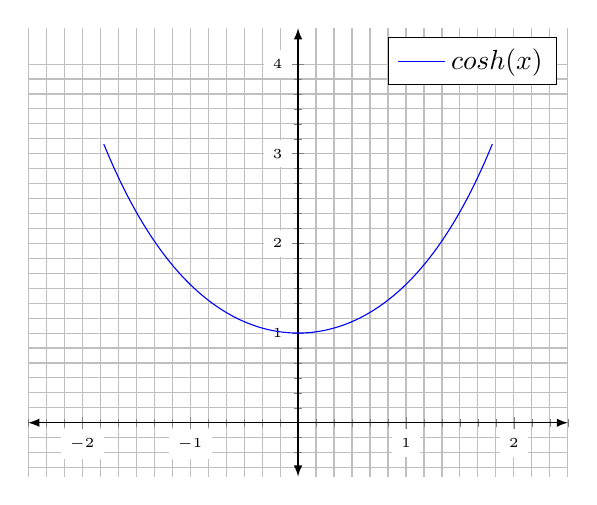
\begin{tikzpicture}
            \begin{axis}[
                    xmin=-2,   xmax=2,
                    ymin=-0.1,   ymax=3.9,
                    grid=both,
                    axis lines=middle,
                    minor tick num=5,
                    enlargelimits={abs=0.5},
                    axis line style={latex-latex},
                    ticklabel style={font=\tiny,fill=white},
                    xlabel style={at={(ticklabel* cs:1)},anchor=north west},
                    ylabel style={at={(ticklabel* cs:1)},anchor=south west}
                ]
                \addplot [
                    domain=-1.8:1.8, 
                    samples=100, 
                    color=blue,
                    ]
                    {cosh(\x)};
                \addlegendentry{$cosh(x)$}
            \end{axis}
        \end{tikzpicture}
        \caption{Représentation graphique de l'équation de la chaînette}
        \label{fig:chainette}
    \end{figure}
    

\subsection{Implémentation}
    L'implémentation d'un \gls{Plugin} \gls{Gazebo} permet de simuler le comportement de l'ombilical dans l'environnement de simulation. Ce \gls{Plugin} est basé sur l'instanciation d'objets de type \textit{Tether} et \textit{TetherElement}. L'objet \textit{Tether} possède les paramètres de simulation de l'ombilical, tandis que l'objet \textit{TetherElement} représente un tronçon de cet ombilical. Un diagramme de classe est présenté en \textsc{Figure}~\ref{fig:uml_class} et montre les différents attributs et méthodes associées à chaque classe.
    
    La \textit{Tether} utilise une structure de liste doublement chaînée\footnote{structure de données liée qui consiste en un ensemble n\oe uds liés les uns aux autres par des références au n\oe uds voisins.} de \textit{TetherElement}. Chaque \textit{TetherElement} possède alors une référence vers l'élément le précédant et l'élément le suivant, comme le montre la \textsc{Figure}~\label{fig:goubly_linked_list}. La \textit{Tether} ne possède ainsi qu'une référence vers le premier et le dernier n\oe ud de la chaîne, nommés respectivements \textit{head} et \textit{tail}. Il est ensuite possible de parcourir la chaîne de \textit{TetherElement} dans les deux sens en utilisant les références gardées par les \textit{TetherElement} eux-mêmes. 

    \begin{figure}[!htb]
        \centering
        \resizebox{0.90\textwidth}{!}{
            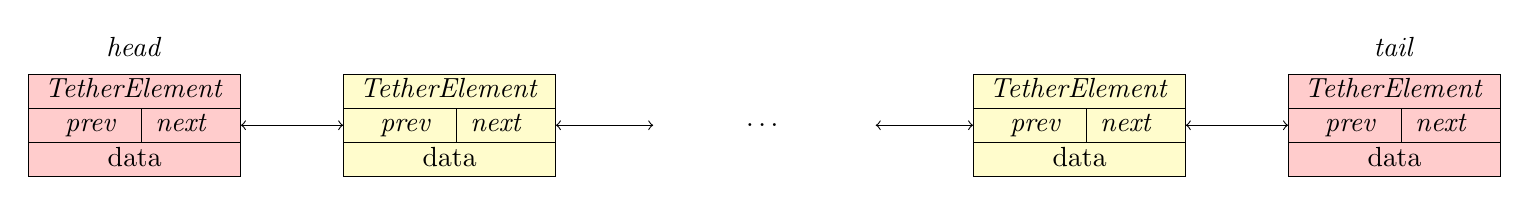
\begin{tikzpicture}
                \tikzset{TE/.style={draw, inner sep=0, outer sep=0, fill=yellow!20}}

                \node[TE, fill=red!20] (TE0) at (0,0) {\begin{tabular}{c} \textit{TetherElement} \\ \hline \hfill \textit{prev} \hfill \vline \hfill \textit{next} \hfill \\ \hline data \end{tabular}};

                \node[TE, fill=red!20] (TE4) at (16,0) {\begin{tabular}{c} \textit{TetherElement} \\ \hline \hfill \textit{prev} \hfill \vline \hfill \textit{next} \hfill \\ \hline data \end{tabular}};

                \foreach \i in {1,3} {
                    \node[TE] (TE\i) at (4*\i,0) {\begin{tabular}{c} \textit{TetherElement} \\ \hline \hfill \textit{prev} \hfill \vline \hfill \textit{next} \hfill \\ \hline data \end{tabular}};
                }
                \node[minimum width=80] (TE2) at (8,0) {\dots};
                \foreach \i in {0,1,2,3} {
                    \pgfmathtruncatemacro{\next}{\i +1}
                    \draw[<->] (TE\i) -- (TE\next);
                }

                \node (head) at (0,1) {\textit{head}};
                \node (tail) at (16,1) {\textit{tail}};
            \end{tikzpicture}
        }
        \caption{Liste doublement chainée}
        \label{fig:doubly_linked_list}
    \end{figure}

    \begin{figure}[!htb]
        \centering
        \resizebox{0.50\textwidth}{!}{
            \begin{tikzpicture}
                \begin{class}[text width=6cm]{Tether}{0,0}
                    \attribute{+ element\_mass : double}
                    \attribute{+ element\_volume : double}
                    \attribute{+ element\_length : double}
                    \attribute{+ position\_first : numpy.ndarray}
                    \attribute{+ position\_last : numpy.ndarray}
                    \attribute{+ elements : list of \textit{TetherElement}}
                \end{class}
            
                \begin{class}[text width=6cm]{TetherElement}{8.5,0}
                    \attribute{+ mass : double}
                    \attribute{+ volume : double}
                    \attribute{+ length : double}
                    \attribute{+ position : numpy.ndarray}
                    \attribute{+ velocity : numpy.ndarray}
                    \attribute{+ acceleration : numpy.ndarray}
                    \attribute{+ previous : TetherElement}
                    \attribute{+ next : TetherElement}
                    \attribute{+ K\_p : double}
                    \attribute{+ K\_d : double}
                    \attribute{+ K\_i : double}
                    \operation{+ F\_p(self) : numpy.ndarray}
                    \operation{+ F\_b(self) : numpy.ndarray}
                    \operation{+ F\_f(self) : numpy.ndarray}
                    \operation{+ Ft\_prev(self) : numpy.ndarray}
                    \operation{+ Ft\_next(self) : numpy.ndarray}
                \end{class}
            
                \aggregation{Tether}{}{~~~n}{TetherElement}
            \end{tikzpicture}
        }
        \caption{Diagramme de classe UML des classes \textit{Tether} et \textit{TetherElement}}
        \label{fig:uml_class}
    \end{figure}

\subsection{Suivi d'angles normalisés}
    Un problème avec la représentation numérique de l'orientation des solides est qu'elle est souvent normalisée, et les valeurs sont ainsi ramenées dans l'intervalle $[-\pi; \pi]$. On ne peut donc pas avoir l'orientation absolue, c'est à dire l'orientation d'un solide en prenant en compte les eventuels tours qu'il aurait pu faire sur lui-même.

    Pour résoudre ce problème, l'\textsc{Algorithme}~\ref{algo:suivi_angle} de suivi d'angles normalisés a été implémenté. Il prends en paramètres l'angle normalisé ainsi que l'angle précédemment calculé, et il retourne la valeur de l'angle absolu. L'idée de fournir l'angle précédent est de pouvoir retourner le nouvel angle qui se trouve dans le même quadrant et aussi de pouvoir suivre les sauts d'angles. Ainsi on peut suivre l'orientation absolue de solides en rotation dans l'espace, en ne fournissant que des orientations relatives ramenées dans l'intervalle $[-\pi; \pi]$, et en gardant en mémoire la précédente orientation calculée.
    
    \begin{algorithm}[!htb]
        \SetKwInOut{Input}{Entrées}
        \SetKwInOut{Output}{Sorties}
        \Entree{$angle\_normalise$, $angle\_absolu$}
        \Sortie{$angle\_absolu$}
        \Deb{
            $offset \leftarrow (angle\_absolu - angle\_normalise + \pi ) \pmod{2\pi}$ \\
            $angle\_absolu \leftarrow angle\_normalise + 2\pi \cdot offset$ \\
        }
        \Retour{$angle\_absolu$}

        \caption{Suivi d'angle} 
        \label{algo:suivi_angle}
    \end{algorithm}

    La \textsc{Figure}~\ref{fig:suivi_angle} présente les résultats de l'\textsc{Algorithme}~\ref{algo:suivi_angle} avec une angle variant dans l'intervalle $[-3\pi; 3\pi]$. On voit sur la première sous-figure l'angle réel et l'angle ramené dans l'intervalle $[-\pi; \pi]$ avec la présence de saut d'angles. Avec cette méthode, on est capable de suivre l'évolution de l'angle et de supprimer cess sauts afin de retrouver l'angle absolu visible dans la deuxième sous-figure et calculé uniquement à partir de la connaissance de l'angle normalisé.

    \begin{figure}[!htb]
        \centering
        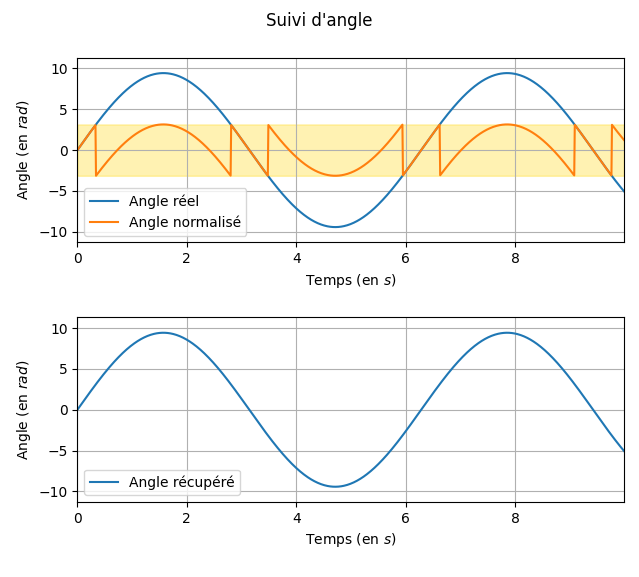
\includegraphics[width=0.5\textwidth]{suivi_angle.png}
        \caption{Suivi d'angle}
        \label{fig:suivi_angle}
    \end{figure}


\subsection{Resultats}
	

	\chapter{Simulation des robots}
	
	\section{Introduction}

		L'environnement dans lequel doivent évoluer les robots à été défini dans le \textsc{Chapitre}~\ref{chapitre:environnement}. Il est maintenant temps de simuler les \gls{ROV}s. Pour ce faire, nous allons devoir décrire les paramètres mécaniques des robots \gls{Argos} et \gls{Atoll}, ainsi que leurs capteurs et actionneurs à simuler.

	\section{Simulation des composants}
		En remarquant que les deux robots embarquent un certain nombre d'éléments communs, il est possible de definir et de simuler les différents composants dans \gls{Gazebo}, afin d'être par la suite chargés dans la simulation des deux robots. La \textsc{table}~\ref{table:components} présente les différents composants à simuler, s'ils nécéssitent l'utilisation d'un \gls{Plugin}, d'une \gls{HardwareInterface} et indique les dépendances entre les robots et ces composants.

		\begin{table}[!htb]
			\centering
			\begin{adjustbox}{max width=\textwidth}
				\begin{tabular}{|l|l|c|c|c|c|}
					\hline
					Composant & Description & \gls{Argos} & \gls{Atoll} & \gls{HardwareInterface} & \gls{Gazebo} \gls{Plugin} \\
					\hline
					\gls{Argos} Frame & Chassis d'\gls{Argos} & \cmark & \xmark & \xmark & \xmark \\
					\hline
					\gls{Atoll} Frame & Chassis d'\gls{Atoll} & \xmark & \cmark & \xmark & \xmark \\
					\hline
					Electronic Pod & Boîtier electronique & \cmark & \cmark & \xmark & \xmark \\
					\hline
					\gls{Latch} & Crochet de levage & \xmark & \cmark & \cmark & \cmark \\
					\hline
					\gls{Navcam} & Caméra de navigation & \cmark & \cmark & \xmark & \cmark \\
					\hline
					\gls{Obscam} & Caméra d'observation & \cmark & \cmark & \xmark & \cmark \\
					\hline
					Rovins & Centrale Inertielle & \cmark & \cmark & \xmark & \cmark \\
					\hline
					Spotlight & Lumières étanches & \cmark & \cmark  & \cmark & \cmark \\
					\hline
					SPE75 Thruster & Propulseur & \cmark & \cmark & \cmark & \cmark \\
					\hline
					SS309 Tilt & Nacelle pour caméra & \cmark & \cmark & \cmark & \cmark \\
					\hline
				\end{tabular}}
			\end{adjustbox}
			\caption{Composants à simuler}
			\label{table:components}
		\end{table}

		Chaque composant a ainsi un \gls{Package} de description qui lui est associe nommé suivant la convention de nommage \gls{ROS} : \textit{component\_description}. Ce package contient tout le code nécéssaire à la description du composant, c'est à dire un modèle \gls{Gazebo} permettant de simuler le composant dans le logiciel de simulation, un fichier de lancement qui s'occupe de lancer le composant dans le simulateur, les \gls{Mesh CAO}. Le code source d'un \gls{Plugin} permettant de décrire le comportement du capteur ou de l'actionneur associé au composant se trouve dans le package \textit{component\_model\_plugin}.

		Nous allons à présent détailler l'implémentation de certains composants qui ont un comportement intéressant à développer.

		\subsection{Latch}

			\subsubsection{Présentation}

				Le Latch est un composant propre au robot \gls{Atoll}. Ce crochet de levage permettant de transporter des structures sous-marines pouvant peser jusqu'à $1,5\ T$ est fabriqué par Forssea Robotics, et permet de positionner et de transporter des balises de positionnement acoustique sur les fonds marins.

			\subsubsection{Hardware Interface}


				
			\subsubsection{Model Plugin}
			
				Un \textit{Model Plugin} a été développé afin de décrire le comportement du \textit{Latch} dans \gls{Gazebo}. Il est basé sur la machine à états finis présenté en \textsc{Figure}~\ref{fig:latch_fsm} et crée un \gls{Joint} entre le \textit{Latch} et la structure à soulever de type encastrement. Les deux solides sont donc attachés l'un à l'autre jusqu'au moment où le signal de relâchement est envoyé au \textit{Latch} simulé, et le \gls{Joint} est alors supprimé.

				\begin{figure}[!htb]
					\centering
					\includegraphics[scale=0.8]{imgs/latch_fsm.pdf}
					\caption{Machine à états du \textit{Latch}}
					\label{fig:latch_fsm}
				\end{figure}

			\subsubsection{Résultats}

				On obtient alors le composant simulable dans l'environnement de simulation \gls{Gazebo}, comme on peut voir sur la \textsc{Figure}~\ref{fig:latch_gazebo}.

		\subsection{SS309 Tilt}

			\subsubsection{Présentation}

				Le \textit{SS309 Tilt} est un composant commercialisé par l'entreprise \textit{Sidus Solutions} et qui permet dans les \gls{ROV}s d'orienter l'\gls{Obscam}. Il est parfaitement étanche et comporte un jeu d'engrenages reliés à un moteur pas-à-pas pilotable en vitesse et en position. On demande ainsi au moteur de mettre l'axe à une certaine position, et l'axe se déplace avec une vitesse de rotation spécifiée.
			
			\subsubsection{Hardware Interface}

			\subsubsection{Model Plugin}

				Pour simuler cet aspect pilotable en vitesse de rotation et position, il faut passer par la simulation d'un moteur pas-à-pas. C'est un moteur un moteur composé de plusieurs bobinages créant ainsi plusieurs phases qui sont allumées succéssivement afin de réaliser une rotation de l'arbre moteur d'un certain incrément d'angle. Cet angle est défini par les caractéristiques du bobinage et n'est donc pas réglable. Il n'est pas non plus possible de piloter précisement la vitesse avec laquelle il se rend à cette position incrémentée. En revanche, il est tout à fait possible de connaître précisement la position du moteur, car l'arbre moteur ne peut prendre qu'un nombre fini d'angles, et il suffit donc de compter le nombre d'incréments commandés. Enfin, on peut commander la vitesse avec laquelle le moteur se rend à cette position, en allumant les phases à la vitesse désirée.

				Nous allons à présent distinguer la position réelle de l'arbre moteur, la position cible et la position commandée. La position réelle est la position de l'arbre moteur dans le simulateur. La position cible est un multiple de l'incrément d'angle à laquelle doit se rendre le moteur à l'instant actuel. La position commandée la position finale dans laquelle doit se retrouver l'arbre moteur et peut être une position réelle quelconque. Le moteur ne sera capable que de se rendre à la position multiple de la valeur de l'incrément d'angle la plus proche de la position commandée. La \textsc{Figure}~\ref{fig:tilt_position} reprends ces différentes notions. En commandant la vitesse à laquelle on incrémente la position cible, on contrôle l'axe en vitesse.

				\begin{figure}[!htb]
					\centering
					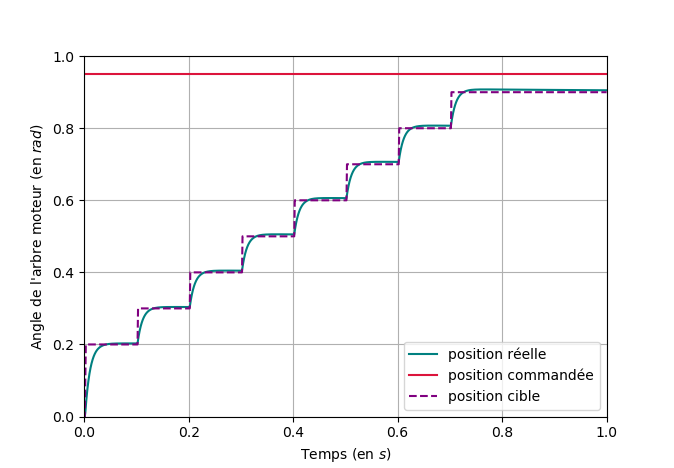
\includegraphics[width=0.6\textwidth]{imgs/stepper_motor.png}
					\caption{Simulation d'un moteur pas-à-pas}
					\label{fig:tilt_position}
				\end{figure}
				
				Pour ce qui est de l'implémentation de ce comportement dans \gls{Gazebo}, on crée un \textit{Thread} qui va s'executer en boucle avec une vitesse variable. Cette vitesse sera fonction de la vitesse de commande du \textit{Tilt} notée $\omega_c$. A chaque tour de boucle, on incrémente donc la position cible de la valeur de l'incrément $d\theta$ si la différence entre la position réelle et la position commandée est plus grande que ce même incrément, et on attends le temps $h$, avec :

				$$h = \frac{d\theta}{\omega_c}$$

				\begin{algorithm}[!htb]
					\caption{Algorithme de simulation d'un moteur pas-à-pas}
					\label{algo:stepper_motor}
					\begin{algorithmic}
						\WHILE {true}
							\STATE read $\theta_r$, $\omega_c$
							\IF {$|\theta_c - \theta_r| > d\theta$}
								\STATE $\theta_t \leftarrow \theta_t + d\theta$
							\ENDIF
							\STATE $h \leftarrow \frac{d\theta}{\omega_c}$
							\STATE sleep $h$
						\ENDWHILE
					\end{algorithmic}
				\end{algorithm}
				

	\section{Simulation d'Argos}

	\section{Simulation d'Atoll}

	% chargement du fichier corps.tex
	% \section{Introduction}

La structure de ce document et certaines parties sont inspir�es de
\cite{guide}.

L'objectif de ce guide est de donner un cadre � l'�criture de rapports 
de projet
� l'\gls{enstab}.
Il vient compl�ter le document d'aide � la
r�daction du rapport de stage op�rateur \og{}Consignes pour la r�daction d'un
m�moire\fg{} disponible sur moodle � l'adresse 
\url{https://moodle.ensta-bretagne.fr/course/view.php?id=408} (section 4). 


La section \ref{sec:gen} pr�sente les g�n�ralit�s sur la nature d'un rapport
de projet. La section \ref{sec:struct} d�crit la structure attendue d'un rapport de
projet.
Puis, la section \ref{sec:regles} d�crit les r�gles m�thodologiques et
typographiques � respecter lors de la r�daction.
Enfin, la section
\ref{sec:outils} offre un aper�u des outils contribuant � l'�criture d'un rapport.


\section{G�n�ralit�s}
\label{sec:gen}

En r�digeant un rapport, vous laissez une trace de votre travail, qui restera
disponible sur le long terme. Il faudra donc veiller � la qualit� du fond
comme de la forme.

Afin d'�tre largement compris, le rapport doit privil�gier une
�criture simple (mais non simpliste) faite de phrases courtes,
employant un vocabulaire explicite. Tous les acronymes doivent �tre explicit�s
et tous les termes techniques expliqu�s.

L'orthographe contribue � l'image que vous laissez de vous-m�me. Si les
correcteurs orthographiques sont d'un usage indispensable, ils ne remplacent
jamais une relecture soigneuse.
De plus, les usages typographiques de la langue employ�e doivent �tre respect�s.

Avant l'entamer la r�daction d'un rapport, les r�ponses � quelques questions
fondamentales sur le rapport vous permettront de cadrer votre travail.

\subsection*{Pourquoi ?}

La r�ponse � cette question permet de d�finir la longueur du
document et son style, et bien entendu la nature du contenu.

\subsection*{Pour qui ?}

La r�ponse � cette question permet de d�finir la teneur des propos, les
notions que le lecteur ma�trise et celles qu'il faut d�tailler. Elle permet
�galement de cibler l'analyse � effectuer. Dans certains cas, elle permet
�galement de fixer le degr� de confidentialit� et
les modalit�s de diffusion.

\subsection*{Pour quand ?}

Cette r�ponse vous permet de g�rer votre temps. Attention, l'�criture de
certaines parties n�cessite un travail de recherche ou d'analyse pr�alable. De
plus, vous 
pouvez avoir � collecter des informations aupr�s de tiers dont vous ne
ma�trisez pas toujours les contraintes.

\subsection*{Pour combien de temps ?}

En r�pondant � cette question, vous allez d�finir la dur�e
d'utilisation du document~; vous en d�duirez l'utilit� d'en g�rer des versions
cons�cutives.


\section{Structure du rapport}
\label{sec:struct}

Il n'y a pas de forme unique et universelle pour un rapport.
N�anmoins, la structure devra toujours comporter des �l�ments qui en
permettent l'utilisation efficace.\index{Structure (rapport)}
Dans tous les cas le rapport devra �tre pagin� et le texte justifi�.

 Le rapport devra \emph{obligatoirement} contenir~:
 \begin{itemize}
 \item un r�sum�~; 
 \item une page titre~;
 \item une table des mati�res~;
 \item une introduction~;
 \item un d�veloppement~; 
 \item une conclusion~;
\item une bibliographie.
 \end{itemize}

%et \emph{pratiquement syst�matiquement}~:
%\begin{itemize}
%\end{itemize}

\emph{Dans la plupart des cas}, on trouvera  �galement~:
\begin{itemize}
\item une liste de mots-cl�s~;  
\item une table des figures ou illustrations~;
\item des remerciements~;
\item une ou plusieurs annexes.
\end{itemize}

\emph{Dans certains cas}, il contiendra enfin~:
\begin{itemize}
\item un index~;
\item un glossaire.
\end{itemize}

Voyons les caract�ristiques de ces diff�rents �l�ments.

\subsection{Page de titre}

La page de titre doit permettre d'identifier le document. Pour cela, elle doit
comprendre~: \index{Page de garde}
\begin{itemize}
\item un titre~;
\item le type du document (par exemple \og{}Rapport de projet\fg{})~;
\item le nom du ou des auteurs du document~;
\item la date de parution (ou de remise du rapport) et �ventuellement le
  num�ro de version~;
\item le nom et le logo de l'organisme dont est issu l'auteur (par exemple
  \textsc{Ensta} Bretagne).
\end{itemize}

\subsection{R�sum�}

Le r�sum� fait la synth�se du projet en une page au maximum. Il
devra contenir une br�ve description du probl�me et des objectifs du projet,
mentionner les r�sultats les plus
importants et dresser une conclusion. Dans le r�sum� il faut surtout mettre en
�vidence les r�sultats car ce sont eux qui rendent mieux compte de votre
travail et donnent l'envie de lire votre rapport. 

Le r�sum� est souvent accompagn� de quelques mots-cl�s et il est, dans
certains cas, traduit en une ou plusieurs langues.\index{Resume@R�sum�}

\subsection{Table des mati�res}

Encore baptis�e \og{} sommaire \fg{}, la table des mati�res permet de
synth�tiser, en d�but de document, les diff�rents chapitres qui y sont
trait�s. Elle doit faire
r�f�rence � la pagination du document pour permettre au lecteur
d'acc�der directement � toute partie du document.\index{Table des
  matieres@Table des mati�res}\index{Sommaire} 

La table des mati�res se g�n�re automatiquement ; ne la cr�ez pas
manuellement, car vous pourriez oublier d'y apporter des
modifications.

\subsection{Introduction}

L'introduction doit permettre de situer le contexte de votre travail. En
particulier, elle doit~:\index{Introduction}
\begin{itemize}
\item pr�senter le contexte de l'�tude~;
\item d�finir le probl�me que le projet cherche � r�soudre, ainsi
    que le cadre dans lequel il s'inscrit~; 
\item d�finir le cadre du travail ; par exemple quelles ont �t� les
  contraintes, la m�thodologie choisie~;
\item annoncer le plan, qui n'est pas un ennonc� plat des diff�rentes parties,
  mais qui vise � d�finir l'orientation de la recherche, les hypoth�ses, le
  cheminement choisi pour tenter de r�pondre � la question.
\end{itemize}

%Il est �galement souhaitable de pr�senter les diff�rentes parties et leur
%encha�nement.

\subsection{D�veloppement}

Le d�veloppement est la partie substantielle de votre document. Il doit �tre
structur� et d�coup� en plusieurs parties. Les encha�nements entre les parties
doivent �tre fluides (par exemple gr�ce � une courte introduction en d�but de
partie et un court bilan � la fin). Il peut s'appuyer sur des compl�ments
d'information (notes de bas de page, r�f�rences, annexes, glossaires ou listes
d'acronymes). N'h�sitez pas � illustrer vos propos par des figures, tables
ou �quations.

\subsubsection{Notes de bas de page}

Les notes de bas de page servent � apporter un compl�ment d'information
non essentiel. Le texte doit pouvoir �tre compris sans y faire appel.
Elles sont tr�s utiles lorsque l'on veut que le document puisse avoir
plusieurs niveaux de lecture.\index{Notes de bas de page}

\subsubsection{Figures et graphiques}

Si on se r�f�re � \cite{tufte}, les graphiques de qualit� doivent
communiquer au lecteur un maximum d'information en un minimum de temps. Lors
de l'utilisation de figures, vous vous attacherez � respecter les r�gles
suivantes~:\index{Figures}
\begin{itemize}
\item Toutes les figures doivent poss�der un titre et �tre cit�es dans le
  document (par exemple \og{}la figure \ref{fig:fract} nous montre que
  \ldots{}\fg{})~; la num�rotation des figures doit �tre g�r�e
  automatiquement.
\item La mise en page doit �tre homog�ne � l'int�rieur d'un graphique.
\item Des graphiques s�par�s servant de base � des comparaisons doivent avoir
  une mise en page coh�rente. Ils doivent notamment �tre repr�sent�s � la m�me
  �chelle et utiliser la m�me palette de couleurs.
\item Selon \cite{tufte}, pour de petits ensembles de
  donn�es\footnote{moins de 20 donn�es}, les 
  tableaux sont plus informatifs que les graphiques.
\item Les graphiques doivent �tre correctement �tiquet�s~:
  \begin{itemize}
  \item si $x$ repr�sente les abscisses et $y$ les ordonn�es, faites en sorte
    que $y=f(x)$ plut�t que $x=f(y)$~;
  \item n'oubliez pas les unit�s sur les axes, typiquement entre crochets
    (voir figure \ref{fig:fract}).
  \end{itemize}
\item Chaque graphique doit �tre analys� dans le corps du document.
\end{itemize}

\begin{figure}[htbp]
  \centering
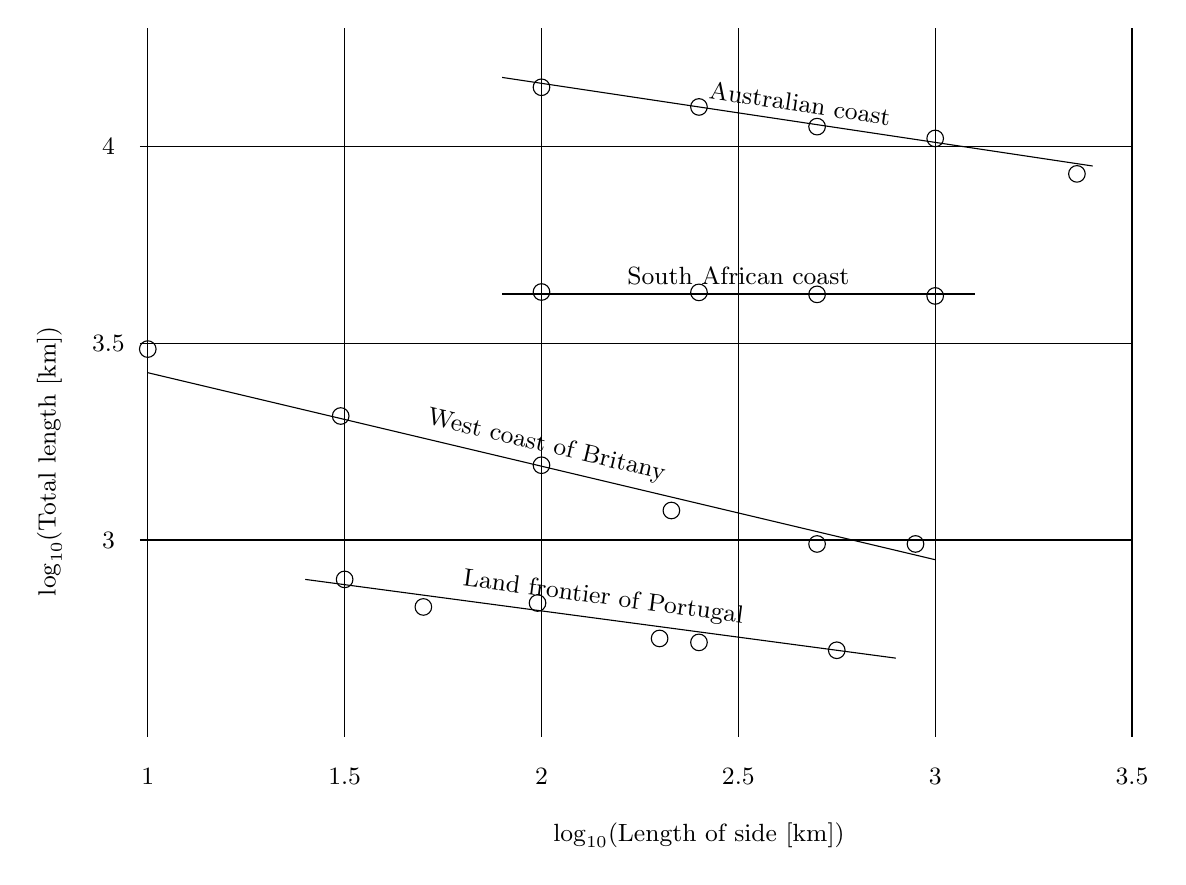
\begin{tikzpicture}[x=1cm,y=1cm,scale=5,font=\small]
  \draw[step=0.5] (0.98,2.5) grid (3.5,4.3);
  \foreach \x/\y in {1/3.485,1.49/3.315,2/3.19,2.33/3.075,2.7/2.99,2.95/2.99,1.5/2.9,1.7/2.83,1.99/2.84,2.3/2.75,2.4/2.74,2.75/2.72,2/3.63,2.4/3.629,2.7/3.624,3/3.62,2/4.15,2.4/4.1,2.7/4.05,3/4.02,3.36/3.93} {
    \draw (\x,\y) circle (0.6pt);
  }
  \draw (1,3.425) -- node[sloped, above] {West coast of Britany}
  (3,2.95);
  \draw (1.4,2.9)-- node[sloped, above] {Land frontier of Portugal} (2.9,2.7);
  \draw (1.9,3.625)-- node[sloped, above] {South African coast} (3.1,3.625);
  \draw (1.9,4.175)-- node[sloped, above] {Australian coast} (3.4,3.95);
  \foreach \x in {1,1.5,...,3.5} {
    \draw (\x,2.4) node {\x};
  }
  \node at (2.4,2.25) {$\log_{10}$(Length of side [km])};
  \foreach \y in {3,3.5,4} {
    \draw (0.9,\y) node {\y};
  }
  \node[rotate=90] at (0.75,3.2) {$\log_{10}$(Total length [km])};
\end{tikzpicture}
  \caption{Dimension fractale de traits de c�te de diff�rents pays ; relation entre longueur et pas}
  \label{fig:fract}
\end{figure}

De mani�re g�n�rale, prenez garde � la lisibilit� de vos figures. Pensez
�galement que la lisibilit� est diff�rente sur �cran, sur une impression
couleur, ou sur une impression en noir et blanc.

Concernant le format des figures, pr�f�rez dans la mesure du possible les
formats vectoriels\footnote{qui ne se d�gradent pas lors des changements de
  taille} comme \emph{eps}, \emph{pdf} ou \emph{svg}. Si vous optez pour un
format image sachez que, de part son algorithme de compression, le format
\emph{jpg} d�gradera fortement le texte~; pr�f�rez-lui le format \emph{png}.

Dans le cas o� la figure est issue d'une capture d'�cran, pensez � ajouter un
habillage et gardez toujours � l'esprit la lisibilit� de la figure~; si
n�cessaire, modifiez les couleurs dans un outil de traitement
d'images\footnote{Par exemple \textsc{gimp}}. 

\subsubsection{Tables}

De la m�me mani�re que les figures, les tables servent � illustrer certains
�l�ments du rapport. Elles doivent poss�der un titre et �tre
r�f�renc�es dans le corps du document. Il faut prendre garde � leur
lisibilit�. Un exemple \emph{� ne pas suivre} est pr�sent� table
\ref{tab:tab1} (table extraite du manuel de \LaTeX). Dans cet exemple, les
lignes (horizontales et verticales) sont 
trop nombreuses et nuisent � la lisibilit�, les alignements sont erratiques,
les unit�s ne sont pas correctement indiqu�es et les nombres sont repr�sent�s
avec des pr�cisions diff�rentes. Enfin, les titres de chaque colonne ne sont
pas apparents.\index{Tables}

\begin{table}[htbp]
  \centering
\begin{tabular}{||l|lr||} 
\hline
\hline
~~~~~gnats     & gram      & 013.65\euro \\ \cline{2-3}
          & each      & .01 \\ \hline
gnu       & stuffed   & 92.5 \\ \cline{1-1} \cline{3-3}
~~~emu       &           & 33.33 \\ \hline
armadillo & frozen    & 8.9887 \\ \hline
\end{tabular}
  \caption{Une table tr�s mal pr�sent�e}
  \label{tab:tab1}
\end{table}

La table \ref{tab:tab2} corrige tous les probl�mes de la table
\ref{tab:tab1}. Cette fois, la table est lisible et elle peut apporter un
compl�ment d'information au texte.

\begin{table}[htbp]
  \centering
\begin{tabular}{@{}llr@{}} 
  \toprule
  \multicolumn{2}{c}{\textbf{Item}} \\ 
  \cmidrule(r){1-2}
  \textbf{Animal} & \textbf{Description} & \textbf{Price (\euro)}\\ 
  \midrule
  Gnat  & per gram  & 13.65 \\
           & each      & 0.01 \\
      Gnu   & stuffed   & 92.50 \\
      Emu   & stuffed   & 33.33 \\
      Armadillo & frozen & 8.99 \\ 
      \bottomrule
\end{tabular}
  \caption{Une table correctement pr�sent�e}
  \label{tab:tab2}
\end{table}

\subsubsection{�quations}

Il est parfois plus simple de d�crire un processus par des �quations que par
du texte. 
De la m�me mani�re que les figures et les tables, les �quations
doivent �tre num�rot�es, et �tre r�f�renc�es dans le texte du
rapport. \index{Equations@�quations}

Exemple~: Soit $S={p_1,\ldots,p_n}$ un ensemble fini de points de
$\nbR^d$. L'�quation \eqref{eq:1} d�crit l'enveloppe convexe de $S$.

\begin{equation}
  \label{eq:1}
  \mathcal C(S)=
  \left\{
    \sum_{i=1}^n\alpha_i p_i \mbox{ avec } \forall i, \alpha_i\geqslant 0
    \mbox{ et } \sum_{i=1}^n\alpha_i =  1
  \right\}
\end{equation}

\subsection{Conclusion}

La conclusion est une syth�se de votre travail et doit en faire un bilan
(critique) vis-�-vis des 
objectifs initiaux. 
Vous devez ici mentionner vos doutes et certitudes quant �
vos r�sultats~; n'h�sitez-pas � fournir des pistes pour un travail � venir ou
des explications pour un travail non abouti.

\index{Conclusion}

\emph{Introduction et conclusion sont des parties essentielles d'un
  document. En les lisant, le lecteur doit pouvoir se faire une id�e
  pr�cise du contenu d�velopp� dans le corps du texte. Il est
  important d'y apporter le plus grand soin.}

\subsection{Bibliographie}

\paragraph{Remarque~:} ce document ne d�crit pas la m�thode
permettant de rechercher des r�f�rences bibliographiques. Pour cela,
reportez vous � l'UV 1.4 \og{}Bibliographie\fg{} accessible sur moodle~:
\url{https://moodle.ensta-bretagne.fr/course/view.php?id=617}.

La bibliographie reprend toutes les r�f�rences qui ont servi de support lors de
votre travail. Elle ne doit contenir que les r�f�rences lues et qui sont
cit�es dans le corps du document.\index{Bibliographie}

Afin de faciliter la maintenance et l'homog�n�it� de la bibliographie, il est
conseill� de s'appuyer sur un outil de gestion de r�f�rences tel que
\emph{Zotero} ou BibTeX. Certains outils\footnote{\emph{Zotero} par exemple,
  mais �galement des sites tels que \url{https://www.diigo.com} ou
  \url{http://www.citethisforme.com}}
permettent une gestion collaborative des r�f�rences.

Exemple~: \emph{Selon \cite{tufte}, pour de petits ensembles de
  donn�es, les tableaux sont plus informatifs que les graphiques.}

L'utilisation de r�f�rences bibliographiques permet~:
\begin{itemize}
\item d'indiquer les r�sultats et conclusions qui viennent d'autres
  travaux (ne pas citer ses sources constitue une faute grave)~;
\item de donner plus de force � vos propos en vous appuyant sur des r�sultats
  reconnus par la communaut� scientifique~;
\item de vous affranchir de l'�criture d'une d�monstration ou d'un calcul~;
\item de citer les documents techniques sur lesquels vous vous appuyez~;
\item de donner des pistes d'exploration pour ceux qui veulent creuser
  certains points.
\end{itemize}

Il existe plusieurs styles classiques de bibliographie, comme par exemple le
format num�rot� dans lequel les r�f�rences sont index�es par un num�ro entre
crochets. Les r�f�rences sont alors ordonn�es selon l'ordre d'apparition dans
le document.

\paragraph{Exemple de bibliographie num�rot�e~:}
\begingroup
\renewcommand{\section}[2]{}%
\begin{thebibliography}{1}
\bibitem{n1} Rudolf \textsc{Bayer} et Edward Meyers \textsc{McCreight}. ``Organization and
  maintenance of large ordered indexes''. In : \emph{Acta Informatica} 1.3
  (1972), p. 173--189.
\bibitem{n3} Beno�t \textsc{Mandelbrot}. ``How long is the coast of Britain ?
  Statistical selfsimilarity and fractional dimension''. In: \emph{Science}
  156.3775 (5 mai 1967), p. 636.
\bibitem{n2} Kenneth Lee \textsc{Clarkson} et al. ``Approximating center points with
  iterated Radon points''. In : \emph{International Journal of
    Computational Geometry \& Applications} 06.03 (sept. 1996), p. 357--377.
\end{thebibliography}
\endgroup

~\\
Un autre format classique est le format alphab�tique dans lequel les
r�f�rences apparaissent dans l'ordre alphab�tique et sont compos�es de lettres
suivies de deux chiffres repr�sentant l'ann�e. Ces lettres sont~:
\begin{itemize}
\item les trois premi�re lettres du nom de l'auteur (s'il est seul)~;
\item les initiales des auteurs (s'ils sont deux ou trois)~;
\item les trois premi�re lettres du nom du premier auteur suivies du symbole
  \og{}+\fg{} (s'il y a plus de 3 auteurs).
\end{itemize}

\paragraph{Exemple de bibliographie alphab�tique~:}
\begingroup
\renewcommand{\section}[2]{}%
\begin{thebibliography}{WWW99}
\bibitem[BM72]{a1} Rudolf \textsc{Bayer} et Edward Meyers \textsc{McCreight}. ``Organization and
  maintenance of large ordered indexes''. In : \emph{Acta Informatica} 1.3
  (1972), p. 173--189.
\bibitem[Cla+99]{a2} Kenneth Lee \textsc{Clarkson} et al. ``Approximating center points with
  iterated Radon points''. In : \emph{International Journal of
    Computational Geometry \& Applications} 06.03 (sept. 1996), p. 357--377.
\bibitem[Man67]{a3} Beno�t \textsc{Mandelbrot}. ``How long is the coast of Britain ?
  Statistical selfsimilarity and fractional dimension''. In: \emph{Science}
  156.3775 (5 mai 1967), p. 636.
\end{thebibliography}
\endgroup

\subsection{Annexes}

Les annexes regroupent les informations qui ne sont pas essentielles � la
compr�hension g�n�rale du rapport et dont la pr�sence dans le texte principal
nuirait � la fluidit� de la lecture. Les annexes peuvent par exemple
contenir~:\index{Annexes}
\begin{itemize}
\item des d�monstrations ou des calculs d�taill�s~;
\item des donn�es techniques (de mat�riel par exemple)~;
\item des donn�es brutes\footnote{uniquement si leur lecture apporte un
    compl�ment d'information utile au lecteur.}~;
\item des glossaires et index.
\end{itemize}

\paragraph{Remarque~:} les programmes offrent rarement un int�r�t dans les
annexes papier. Par contre, il peut �tre int�ressant de les joindre sous forme
num�rique\footnote{Par exemple dans un fichier archive \emph{7z}, \emph{tgz},
  \emph{tbz}, \emph{zip} ou \emph{rar}.}.

\subsection{Index et glossaire}

L'index et le glossaire sont plac�s dans les derni�res pages du
document. L'index permet de retrouver les termes cl�s du document par une
recherche alphab�tique~; il acc�l�re la recherche d'information dans les
rapports volumineux.\index{Index}

Le glossaire permet de regrouper la description de termes techniques et de
sigles � la fin du document. Il permet une meilleure compr�hension des
concepts dont l'explication n'est pas reprise en d�tail dans le texte.\index{Glossaire}

\section{R�gles}
\label{sec:regles}

\subsection{R�gles m�thodologiques}

Le document doit �tre consid�r� comme un tout homog�ne et non comme
une compilation d'�l�ments disparates. Les auteurs sont solidairement
responsables (en contenu et en d�lai) de la totalit� du document et
non uniquement de leur propre contribution.\index{Methodologie@M�thodologie}

La coh�rence doit �tre recherch�e � tous les niveaux afin de limiter
les ambigu�t�s et d'am�liorer la qualit� du document produit. Avant la remise
d'un rapport cons�quent, plusieurs phases de relecture sont g�n�ralement
n�cessaires. Il est donc conseill� de commencer l'�criture du rapport d�s que
possible. 

On veillera tout particuli�rement �~:
\begin{itemize}
\item respecter la coh�rence du style, des  temps et des modes employ�s ;
\item conserver le m�me mode de locuteur dans tout le texte (p.~ex.
  je, nous, l'�quipe) ;
\item utiliser le m�me niveau de vocabulaire tout au long du texte. 
\end{itemize}

\subsection{R�gles de typographie}

Les usages de typographie diff�rent d'une langue � l'autre. Si le rapport est
�crit en anglais, vous devez alors respecter les usages
anglo--am�ricains~; consultez par exemple \cite{typoUS} pour des
informations d�taill�es. \index{Typographie}

De m�me, dans tous les cas o� vous �crivez votre rapport en
fran�ais, il est important de respecter les r�gles de typographie fran�aise.
Dans ce cas,
la lecture de \cite{andreTypo} vous donnera un tr�s bon aper�u des r�gles
� respecter et des �cueils � �viter.

\subsection{R�gles de pr�sentation de r�sultats num�riques}

Sauf dans le cas de valeurs dimensionnelles, les unit�s des r�sultats
num�riques doivent toujours �tre pr�cis�es. 

Il est �galement important d'�tre conscient du sens implicite donn� lors de la
pr�sentation de valeurs num�riques. En particulier, le nombre de chiffres
significatifs pr�sent� traduit la fid�lit� de la mesure. Les chiffres
significatifs excessifs doivent �tre supprim�s par arrondi.

\section{Outils d'aide � la production de documents}
\label{sec:outils}

Lors de votre scolarit� � l'\gls{enstab}, vous avez g�n�ralement le
choix des outils utilis�s pour la production de documents. 

\subsection{Traitement de texte et formateur de texte}

Un traitement de texte est un outil de mise en page de documents. Il est
g�n�ralement de type \gls{wysiwyg}\footnote{What You See Is What You Get}
et permet donc de voir l'aspect du document se modifier en continu. Dans cette
cat�gorie, les outils les plus connus sont \emph{Microsoft Word} et
\emph{LibreOffice}. Le formatage du texte est
obtenu par application de {\em styles}. Malheureusement, de nombreux
utilisateurs, insuffisamment form�s, n'utilisent pas ou utilisent mal
cette fonctionnalit�.

Le formateur de texte le plus connu est \LaTeX. Il proc�de en s�parant le fond
et la forme du document et poss�de des biblioth�ques de style qui permettent
de respecter les r�gles typographiques. Cet outil est g�n�ralement
non-\gls{wysiwyg} et requiert un certain investissement avant d'�tre
utilis� efficacement.

\subsection{Format des donn�es}

La question du format de donn�es se pose obligatoirement lors de la
manipulation de documents num�riques. Le choix du format est souvent li� �
l'outil utilis�. Dans la mesure du possible, il est conseill� d'utiliser des
formats ouverts (c'est-�-dire dont la sp�cification est disponible).
Cette question est particuli�rement importante lors du partage de document.

Voici quelques conseils pour vous aider dans le choix du format de donn�es~:
\begin{itemize}
\item lors de la remise de documents \emph{non modifiables}, destin�s � des
  sorties papier, il est conseill� d'utiliser le format \emph{pdf}~; soyez
  vigilants � l'int�gration des polices de caract�res lors de la g�n�ration et
  v�rifiez syst�matiquement le r�sultat~; 
\item pour des documents consultables en ligne, le format \textsc{Html}
  conviendra parfaitement~;
\item pour l'�change de documents � modifier, les formats \emph{odt},
  \emph{rtf} et \emph{tex} sont ouverts~;
\item en ce qui concerne le format \emph{docx}, les sp�cifications existent,
  mais ne sont pas exactement respect�es par \emph{Microsoft Word}, ce qui
  entra�ne des probl�mes de mise en page lors du passage par
  \emph{LibreOffice}\ldots{} Dans ce cas, il faudra veiller � ce que tous les
  r�dacteurs utilisent la m�me version de \emph{Microsoft Word} ou de
  \emph{LibreOffice}. 
\end{itemize}

\subsection{Outils collaboratifs}

R�diger un rapport � plusieurs est toujours une op�ration
d�licate. L'utilisation d'outils collaboratifs permet de simplifier cette
phase, de manipuler plusieurs versions du document et de g�rer les conflits.
Plusieurs solutions sont disponibles~:
\begin{itemize}
\item utiliser le mode \og{}Modifications\fg{} de \emph{Microsoft Word} ou de
  \emph{LibreOffice}~; l'�change de fichiers et la gestion de version doivent
  alors �tre assur�s manuellement~;
\item utiliser un gestionnaire de version\footnote{Par exemple du \textsc{cvs}
  ou du \emph{subversion} h�berg� sur le serveur
  \url{https://gforge.ensta-bretagne.fr/gf} ou une gestion d�centralis�e avec
  \url{https://github.com}.} pour h�berger le code source
\LaTeX\footnote{Cette m�thode ne fonctionne que si le document est au format
  texte.}~;
\item h�berger le rapport sur un service \emph{cloud} tel que
  \emph{Google drive} ou \emph{Microsoft Office 365}.
\end{itemize}

\section{Conclusion}

Dans ce guide, les objectifs d'un rapport de projet ont
�t� pr�cis�s ainsi que la structure classique de son plan. Ensuite,
les r�gles de base pour sa r�daction ont �t� pr�sent�es, suivies d'un
rapide traitement des probl�matiques li�es aux outils de production de
documents. 



%%% Local Variables: 
%%% mode: latex
%%% TeX-master: "../guide"
%%% End: 


	\appendix

	\clearpage

	\phantomsection
	\addcontentsline{toc}{section}{Liste des tableaux}
	\listoftables

	\clearpage
	\phantomsection
	\label{sec:index}
	\addcontentsline{toc}{section}{Index}
	\printindex


	\printglossaries


	\clearpage
	\phantomsection
	\addcontentsline{toc}{section}{Bibliographie}

	\bibliography{bib/sea}
	\bibliographystyle{alpha}

\end{document}
